\documentclass[smaller,handout,table]{beamer}

\usetheme{clecturesty}

\subtitle{Lecture 5 of 5}

\begin{document}

{
\logo{
\includegraphics[width=0.30\textwidth]{imperialblue}}
\begin{frame}
  \titlepage
\end{frame}
}


\section{Function Pointers}
\subsection{Last Week...}
\begin{frame}{Last Week...}
\begin{itemize}
\item Arrays in C are not limited to two dimensions.
\item We can create our own data types using \kw{struct}s.
\item Global variables can be accessed anywhere in your program.
\item The lifetime of a variable can be extended by making it \kw{static}.
\item A 'Release' build will optimise your program during compile-time.
\item Using the bits that make up individual data types can be an efficient alternative the data types themselves.
\end{itemize}
\end{frame}


\subsection{Pointers IV - Functions Pointers}
\begin{frame}[fragile]
\frametitle{More Pointers!}
\begin{itemize}
\item So far, we have seen examples of pointers to:
\begin{itemize}
\item native types (such as {\tt\kw{int}*}, {\tt\kw{float}*}, {\tt\kw{double}*}...)
\item something unknown, which we \textit{can} recast ({\tt\kw{void}*})
\item structures (such as {\tt FILE*})
\item and pointers themselves (such as {\tt\kw{int}**}, {\tt\kw{double}**}...)
\end{itemize}
\item There is one more pointer type, a pointer to a \emph{function}.
\end{itemize}

\begin{block}{Why point to functions?}
C code is often re-used between projects. Mathematical routines such as ones to find roots of functions, become extremely limited if they are tied down to a specific case.
\end{block}

\begin{exampleblock}{Declaring a pointer to a function}
We do this with a {\tt\kw{typedef}}:
\vspace{-0.1in}
\begin{center}
\tt \kw{typedef} \kw{double} (* fx)(\kw{double} x);
\end{center}
\end{exampleblock}
\end{frame}

\subsection{Example of a Function Pointer}
\begin{frame}[fragile]
\frametitle{Function Pointers - An example}
\vspace{-0.2in}
\begin{semiverbatim}
\tiny
\kw{\#include} \kt{<stdio.h>}
\kw{typedef double} (* fx)(\kw{double} x);

\kw{double} newtonSolve(fx func, fx grad, \kw{double} guess)
\{
   \kw{unsigned int} loop;
   \kw{for} (loop = 0; loop < 10; loop++) guess -= func(guess)/grad(guess);
   \kw{return} guess;
\}

\kw{double} sample(\kw{double} x)
\{
   \kw{return} x*x-2.0;
\}

\kw{double} dsample(\kw{double} x)
\{
   \kw{return} 2.0*x;
\}

\kw{int} main()
\{
   \kw{double} sol = newtonSolve(sample, dsample, 1.0);
   printf(\kt{"Solution = \%.15lg\\n"}, sol);     
   printf(\kt{"Residue = \%lg\\n"}, sample(sol));
   \kw{return} 0;
\}
\end{semiverbatim}
This should get you started with exercise \# 5.
\end{frame}

\section{Using Existing Code}
\subsection{Don't Do it All Yourself!}
\begin{frame}
\frametitle{Don't Do it All Yourself!}
\begin{itemize}
\item As you have seen from the exercises, writing functions to solve equations such as cubics can become complicated (especially when rounding error needs to be minimised).
\item A lot of people have spent a considerable amount of time attempting to perfect implementations of mathematical functions.
\item Routines written by a third party are packaged in \emph{libraries}.
\item These are available for you to link your program with.
\end{itemize}
\end{frame}

\subsection{Converting Fortran}
\begin{frame}
\frametitle{Using Fortran Code}
\begin{itemize}
\item In addition to libraries, there is existing source code that can be used...
\item Scientific programming has been going on for $\approx 70$ years (counting from Colossus) in Britain.
\item Unfortunately a lot of this has been carried out in Fortran.
\end{itemize}
\begin{block}{\tt f2c}
Bell Labs have released a program called {\tt f2c} which converts Fortran source code to C. The output from {\tt f2c} is usually not very human friendly, but it does at least compile.
\end{block}
\end{frame}

\subsection{Scientific Libraries}
\begin{frame}
\frametitle{GNU Scientific Library - GSL}
GNU have released their C Scientific Library:
\begin{center}
\url{http://www.gnu.org/software/gsl/}
\end{center}

\begin{itemize}
\item It is managed by scientists at Los Alamos, and is very comprehensively documented.
\item GSL requires gcc (but ``ports'' are available - Windows users, see the handouts on my web page)
\end{itemize}

\begin{alertblock}{Licensing}
``GSL can be used internally (`in-house') without restriction, but only redistributed in other software that is under the GNU GPL.''
\end{alertblock}
\end{frame}

\begin{frame}[fragile]
\frametitle{GSL Example}
\vspace{-0.2in}
\begin{semiverbatim}
\small
\kw{\#include} \kt{<stdio.h>}
\kw{\#include} \kt{<gsl/gsl\_sf\_bessel.h>}

\kw{int} main()
\{
   \kw{double} x = 0.0;

   printf(\kt{"Enter x \\n"});
   scanf(\kt{"\%lf"}, \&x);
   printf(\kt{"J0(\%g) = \%.18e\\n"}, x, gsl\_sf\_bessel\_J0(x));

   return 0;
\}
\end{semiverbatim}
Compile this using the command-line (assuming you have GSL installed):
\begin{verbatim}
gcc gsl-sample.c -lgsl  -lgslcblas -lm -o gsl-sample
\end{verbatim}
\end{frame}

\begin{frame}
\frametitle{NAGLIB}
The Numerical Algorithms Group, based in Oxford, maintain a software library called NAGLIB.
\begin{itemize}
\item Certain departments in Imperial College have a license for this.
\item Check with the Software Shop; you might be covered.
\end{itemize}
\end{frame}

\begin{frame}
\frametitle{General Numerical Software}
\begin{center}
\begin{columns}
\begin{column}{0.3\textwidth}

\includegraphics[width=\textwidth]{netlib.png}\\
\end{column}
\end{columns}
The Netlib Repository contains a lot of very useful numerical code and papers. It is definitely worth having a route through their website:\\
\url{www.netlib.org}
\end{center}
\end{frame}

\section{Parallel Computing}
\subsection{Parallel Computing}
\begin{frame}{Parallel Computing}
\begin{block}{What is Parallel Processing?}
\begin{list}{$\bullet$}{}
\item The programs we have been creating compile to machine code which is passed (serially) through a processor.
\item Modern desktop computers no longer have just one processor with one processing core within it. They have one or more, multi-cored processors.
\item This means there is the ability to run multiple `threads' of a program, each one on its own core, allowing us to take advantage of the full power of the processor.
\item There are a few ways to utilise multiple processors, but it can't be done for all code/algorithms.
\end{list}
\end{block}
\end{frame}

\begin{frame}[fragile]
\frametitle{How many processors do I have?}
\begin{block}{}
\begin{columns}
\begin{column}{4cm}
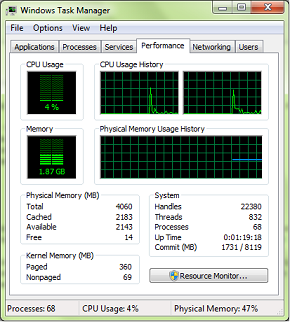
\includegraphics[width=\textwidth]{taskman.png}
\end{column}
\begin{column}{6cm}
In Windows press \\\texttt{[Ctrl] + [Shift] + [Esc]} \\to open Task Manager, then look at the ``Performance'' tab.
\end{column}
\end{columns}
\end{block}
\begin{block}{}
In Linux run:
\begin{semiverbatim}
grep -c "^processor" /proc/cpuinfo
\end{semiverbatim}
\end{block}
\end{frame}

\begin{frame}{Ways to utilise Multiple Processors}
Wherever our code is running a loop (i.e. doing the same thing across a large data range) we can start to think about parallel execution.\\
I'm going to mention three of the many ways to take full advantage of your processor:
\begin{enumerate}
\item Running multiple instances of the program.
\item Running threads in a shared memory environment.
\item Using MPI in a distributed memory environment.
\end{enumerate}
\end{frame}

\begin{frame}{1. Running Multiple Instances}
\begin{list}{$\bullet$}{}
\item Running multiple instances of a serial program is the simplest way to use more than one processor.
\item We simply write our code as normal and start $n$ instances of it at the same time, with $n$ being the number of cores to use.
\item If your program is running across multiple discrete datasets - for example, processing multiple output files from another program - then running multiple instances, each one targeting separate datasets, might be effective.
\item This is only appropriate when no data needs to be shared between processes.
\end{list}
\end{frame}

\begin{frame}{2. Threads in Shared Memory}
\begin{list}{$\bullet$}{}
\item Within a program, one can spawn multiple execution threads.
\item Threads are all owned by the parent process but are running independently. They can each access their own and shared memory.
\item Threads can be spawned arbitrarily, but are particularly useful for splitting up parts of \texttt{\kw{for}} loops between cores and running them in parallel.
\item Because running loops in parallel means that they no longer execute sequentially, only algorithms where an iteration does not rely on another can be run in this way.
\item Threads in shared memory (not surprisingly) require shared memory. As a ``rule of thumb'' this is available anywhere where the processors sit in the same physical box.
\item We will look at simple use of OpenMP to make our programs run in this way.
\end{list}
\end{frame}

\begin{frame}{3. MPI in Distributed Memory}
\begin{list}{$\bullet$}{}
\item Multi-threaded code for shared memory could alternatively be coded for distributed memory.
\item A Distributed Memory System is one in which not all processors are addressing the same memory. A common scenario would be using more than one node in a computation cluster.
\item Parallel code for distributed memory requires using a Message Passing Interface to send information between the threads/processes.
\item This is often more difficult as (unlike with OpenMP) the initial single-threaded code needs to be restructured.
\item Programs using MPI can be used on shared and distributed memory systems alike.
\item Using MPI is beyond the scope of this course, but you may wish to investigate it for future projects.
\end{list}
\end{frame}

\subsection{Multi-Threading with OpenMP}
\begin{frame}{OpenMP}
\begin{block}{}
OpenMP (Open Multi-Processing) is an API (Application Programming Interface) that can be used to create a multi-threaded program in shared memory with only minor modifications to your initial, single-threaded program.
\end{block}
\begin{block}{}
It is included with the majority of compilers. In \texttt{gcc} use the \texttt{-fopenmp} switch to enable OpenMP. For Visual Studio or Code::Blocks see the information sheets on my web page.
\end{block}
\begin{block}{}
Multi-threading, and the use of OpenMP, are large topics. We will just cover the use of OpenMP to run \texttt{\kw{for}} loops in parallel; this should be sufficient to create efficient, parallel code for a large number of applicable algorithms.
\end{block}
\end{frame}

\begin{frame}{Writing Multi-Threaded Code}
\begin{enumerate}
\item Write your algorithm, running on a single thread.
\item Compile, debug and thoroughly test you code.
\item Identify regions that could run in parallel - look for \texttt{\kw{for}}s!
\item Add OpenMP compiler directives.
\item Compile with OpenMP support.
\end{enumerate}
\end{frame}

\begin{frame}[fragile]
\frametitle{When Can We Multi-Thread?}
When one iteration does not depend on another.
\begin{block}{Bad Examples}
\begin{semiverbatim}
\krr{8}\kl\kw{for}(i = 1; i <= n; ++i)  \kc{//Loop 1}
\kl a[i] = a[i-1] + b[i];

\krr{5}\kl\kw{for}(i = 0; i < n; ++i)   \kc{//Loop 2}
\kl x[i] = x[i+1] + b[i];
\end{semiverbatim}
\end{block}
\begin{block}{}
The two above examples could not be run in parallel:
\begin{list}{$\bullet$}{}
\item The first example requires the previous iteration to be finished before it can run the next.
\item The second could not be run in parallel as another thread might change the original value of $x[i+1]$ before it has been used to calculate $x[i]$.
\end{list}
\end{block}
\end{frame}

\begin{frame}[fragile]
\frametitle{Using OpenMP}
To make a \texttt{\kw{for}} loop run on multiple cores, use the \texttt{parallel for} OpenMP compiler directive on the line above:
\begin{semiverbatim}
\krr{6}\kl\kw{#pragma} omp parallel for
\kl\kw{for} (i = 0; i < max\_i; i++)
\kl \{
\kl     a[i] = b[i] + c[i+1];
\kl \}
\end{semiverbatim}
This will automatically split up the \texttt{\kw{for}} loop, and run it on all available cores.
\end{frame}

\begin{frame}[fragile]
\frametitle{Private and Shared Variables}
\begin{block}{}
By default all variables are shared, this means any thread has access to them. There are three exceptions:
\begin{list}{$\bullet$}{}
\item The loop index.
\item Variables that are declared within the for loop.
\item Variables explicitly listed as private or a reduction.
\end{list}
\end{block}
\begin{block}{}
No other thread can read or write to another thread's private variables. This is important for loop indexes as each thread needs to keep track of its own position in the loop. It is also useful for intermediate values in a calculation
\end{block}
\begin{block}{}
To explicitly list a variable such as \texttt{sqrt\_q} as private we modify our compiler directive:
\begin{semiverbatim}
\kw{#pragma} omp parallel for private(sqrt\_q)
\end{semiverbatim}
\end{block}
\end{frame}

\begin{frame}[fragile]
\frametitle{Reductions}
\begin{block}{}
Two threads modifying the same variable at the same time can cause problems. To overcome this potential problem we can use a ``reduction''. A reduction makes a variable private in each thread and then uses a rule operator (\verb#+,-,*,|,&,^,&&#) to reduce all the private values back to the original variable after the for loop.
\end{block}
\begin{block}{An Example}
\begin{semiverbatim}
\krr{6}\kl\kw{int} i = 1, factorial;
\kl\kw{#pragma} omp parallel for reduction(*: factorial)
\kl\kw{for} (i = 1; i <= x; i++)
\kl\{
\kl    factorial *= i;
\kl\}
\end{semiverbatim}
\end{block}
\end{frame}

\begin{frame}[fragile]
\frametitle{Bringing it all together: An Example}
\begin{small}
\begin{block}{Single-Threaded Loop}
\begin{semiverbatim}
\krr{5}\kl\kw{int} **Matrix, i, col, sum;
\kl\kw{for} (i=0; i<rows; i++)
\kl\{
\kl     col = WhichColumn(i);
\kl     sum += Matrix[i][col];
\kl\}
\end{semiverbatim}
\end{block}
\begin{block}{Multi-Threaded Loop}
\begin{semiverbatim}
\krr{5}\kl\kw{int} **Matrix, i, row, sum;
\kl\kw{#pragma} omp parallel for private(col) reduction(+: sum)
\kl\kw{for} (i=0; i<rows; i++)
\kl\{
\kl     col = WhichColumn(i);
\kl     sum += Matrix[i][col];
\kl\}
\end{semiverbatim}
\end{block}
\end{small}
\end{frame}

\subsection{High Performance Computing}
\begin{frame}{High Performance Computing}
\begin{block}{}
\begin{list}{$\bullet$}{}
\item Once you have made a good multi-threaded program, if it is still taking a long time to compute and you need results faster, you may wish to run it on an HPC.
\item An HPC is a large computing cluster containing many, many, fast processors across multiple nodes (physical computers).
\item Threading in shared memory can utilise all the processors in one node, code using MPI can be run across multiple processors and multiple nodes.
\item Imperial College has a very large HPC and CPU time can be rented from them, for information see:\\
\url{http://www3.imperial.ac.uk/ict/services/hpc}
\end{list}
\end{block}
\end{frame}

\section{Other Programming Languages}
\subsection{C++}
\begin{frame}
\frametitle{Moving on to C++}
\begin{block}{What is it?}
\begin{itemize}
\item C++ can be thought of very loosely as an object oriented extension to C.
\item The C++ standard is over twice as big as the C standard.
\item C++ is still actively developed and maintained.
\end{itemize}
\end{block}
\begin{exampleblock}{References}
\begin{columns}
\begin{column}{1.7cm}

\includegraphics[width=\textwidth]{deitelnew.jpg}
\end{column}
\begin{column}{8cm}
\begin{itemize}
\item One good book that has been brought to my attention is ``C++ How to Program, 8th Edition'' by Harvey and Paul Deitel published in 2011.
\item Before buying any C++ book, make sure that it is recent, and that you like the writing style.
\end{itemize}
\end{column}
\end{columns}
\end{exampleblock}
\end{frame}

\subsection{C\#}
\begin{frame}
\frametitle{Moving on to C\#}
C\# belongs to a different class of language.
\begin{itemize}
\item C\# targets the .NET framework. This can be thought of as an \textbf{extensive} library of well-maintained and (mostly) stable general-purpose functions.
\item .NET runs in software, rather than directly on hardware. This results in slower code, but a consistent and safe execution environment.
\item C\# is \textit{my} language of choice. The language, together with .NET, favours fast and intuitive development of powerful programs.
\item Pointers are hidden from the user in C\#. Most memory allocation and de-allocation is done automatically, via \emph{garbage collection}.
\item To combine the execution speed of C and the development power of C\# I have previously written fast algorithms into C libraries and written a program around it in C\#.
\item C\# is less portable than C; C\# can only be run on .NET for windows, or Mono for Linux, Mac, Android and iOS.
\end{itemize}
\end{frame}

\begin{frame}
\frametitle{C\# References}
\begin{block}{Book}
\begin{columns}
\begin{column}{1.7cm}

\includegraphics[width=\textwidth]{csharp.png}
\end{column}
\begin{column}{0.8\textwidth}
\begin{itemize}
\item ``Pro C\# and the .NET 4.5 Framework, 6th Edition'' by Andrew Troelsen,
appears to be up-to-date and comprehensive.
\end{itemize}
\end{column}
\end{columns}
\end{block}
\begin{exampleblock}{MSDN}
The definitive (and free) source of information for Microsoft Platforms is the MSDN, the C\# documentation is browsable at:\\
{\small\url{http://msdn.microsoft.com/en-gb/library/kx37x362.aspx}}
\end{exampleblock}
\end{frame}

\section{Summary}
\subsection{Summary}
\begin{frame}{Summary}
\begin{list}{$\bullet$}{}
\item We can create pointers to functions. This enables us to pass functions to another function.
\item There exist function libraries that you can use rather than write your own versions of established algorithms.
\item By running multiple instances of your program, or writing a multi-threaded program, you can use the full processing power of your computer.
\item An HPC is a very powerful computer-processing cluster and can be hired to run CPU intensive code.
\end{list}
\end{frame}

\end{document}
